\documentclass[10pt,aspectratio=169]{beamer}

\usepackage[sfdefault]{roboto}
\usepackage[utf8]{inputenc}
\usepackage[T1]{fontenc}

\usepackage{styles/fluxmacros}
\usefolder{styles}

% Available style: asphalt, blue, red, green, gray 
\usetheme[style=asphalt]{flux}

\usepackage{booktabs}
\usepackage{colortbl}
\usepackage{ragged2e}
\usepackage{schemabloc}
\usepackage{hyperref}
\usepackage{ragged2e}
\usepackage{comment}
\usepackage[ddmmyyyy]{datetime} 
\usepackage{longtable}
\usepackage{anyfontsize}
\usepackage{framed}
\renewcommand{\dateseparator}{.}

%\usebackgroundtemplate{
%
\includegraphics[width=\paperwidth,height=\paperheight]{assets/background.jpg}}%change this to your preferred background for the presentation.

\definecolor{bgcolor}{HTML}{222222}
\setbeamercolor{background canvas}{bg=bgcolor}

\let\raggedright=\RaggedRight
\hyphenation{TensorFlow Experiment-Impact-Tracker Objekt-erken-nung energie-ef-fi-zienten}

\title{\Large Was weiß ChatGPT über Nachhaltige Software-Entwicklung}
\subtitle{\Large und Green Coding? Erste Tests und Bewertungen}
\author{\large Stefan Naumann, Achim Guldner, Sebastian Weber und Max Westing}

% DATUM in Datei: beamerouterthemeflux.sty
% Fuszeilen-Titel: dito

\institute{\\Hochschule Trier\\Umwelt-Campus Birkenfeld\\Institut für Softwaresysteme}
\titlegraphic{assets/logoucb.pdf}
%~~~~~~~~~~~~~~~~~~~~~~~~~~~~~~~~~~~~~~~~~~~~~~~~~~~~~~~~~~~~~~~~~~~~~~~~~~~~~~

\begin{document}
\titlepage

%\begin{frame}{Agenda}
%	\tableofcontents
%\end{frame}

% Einführung und Ziele
% Method
% Experiments
% Results
% Discussion

\section{Einführung und Ziele}
\begin{frame}{Einführung und Ziele}
    \begin{minipage}{0.65\linewidth}
    \begin{itemize}
        \item Die Veröffentlichung von ``ChatGPT'' hat erhebliche Aufmerksamkeit erzeugt
        \item Google Scholar: ``about'' 33.700 Ergebnisse für den Begriff ``ChatGPT''
        \item Offene Fragen: wissenschaftliche Qualität der ChatGPT-Ergebnisse und potenzielle Einschränkungen
        \item Ziele
        \begin{itemize}
            \item ChatGPT (Version GPT-3.5) zu Themen ``Nachhaltige/Grüne Software-Entwicklung'' (GSE) bzw. ``Green Coding'' (GC) zu befragen
            \item Einschätzung wie Sprachmodelle die Forschung in GSE/GC unterstützen können
            \item Potenzielle Vorteile und Risiken in Forschung und praktischen Anwendungen diskutieren
        \end{itemize}
    \end{itemize}
    \end{minipage}
    \begin{minipage}{0.34\linewidth}
        ~~~~~~~~
\includegraphics[width=0.9\textwidth]{assets/AdobeStock_562926073_sm.jpeg}

        \tiny
        ~~~~~~~~~ Bild: \hyperlink{https://stock.adobe.com/de/images/ai-copy-writing-bot-artificial-intelligence-copywriter-bot-using-chatgpt-by-open-ai-for-content-writing-holding-pencil/562926073}{Adobe Stock | \#562926073}
    \end{minipage}
\end{frame}



\section{Stand der Technik}
\begin{frame}{Stand der Technik}
    \begin{itemize}
        \item LLMs: leistungsstarke Sprachmodelle mit Millionen von Parametern
        \item Vielfältige Aufgaben in der natürlichen Sprachverarbeitung
        \item Daher: Wandel in Natural Language Processing~-~NLP, von spezialisierten zu universelleren Modellen
        \item Weitere Chat-Tools: HuggingChat, BARD; Weitere Modelle: BERT, LLaMA, PaLM
        \item Integration dieser Tools in Forschung und Bildung oft im Dialog mit Chatbots untersucht
        \item Google's Tailwind: Modelle für spezifische Anwendungsfälle anpassen
        \item Bedenken/Risiken: Sicherheit, Black-Box, "Halluzinationen": falsche oder erfundene Informationen, die aber als Fakten dargestellt werden
        \item Außerdem: Enormer Energie- und Ressourcenaufwand für Training und Inferenz
        \item Keine Informationen zu Umweltauswirkungen von GPT, ca. 50,5 Tonnen $CO_2$-Äquivalente für ein BLOOM-Modell mit 176 Milliarden Parametern
    \end{itemize}
\end{frame}

\section{Vorgehen}
\begin{frame}{Vorgehen}
    Input-Prompts an ChatGPT
    \small
    \begin{longtable}{|p{6.85cm}|p{6.85cm}|}
    %\multicolumn{2}{|l|}{\textbf{Sprache}} & \multicolumn{2}{|l|}{\textbf{Version}}\\\hline
    \hline
    \textbf{Deutsch}                                                                       & \textbf{Englisch}\\\hline
    Was ist Green Coding?                                                                  & What is Green Coding? \\\hline
    Was ist Green Software Engineering?                                                    & What is Green Software Engineering?  \\\hline
    Kennst Du Definitionen (von Green Software Engineering) aus wissenschaftlichen Papern? & Do you know definitions (of Green Software Engineering) from scientific papers?          \\\hline
    Wie viel Energie benötigt Software?                                                    & How much energy does software need? \\\hline
    Wie kann man den Energiebedarf von Software messen?                                    & How to measure the energy consumption of software?  \\\hline
    Wie kann man Software ressourceneffizienter machen?                                    & How to make software more resource efficient? \\\hline
    Ich brauche ein Referenzmodell für Nachhaltige Software.                               & I need a reference model for green
    software.  \\\hline
    Was sind die wichtigsten wissenschaftlichen Quellen zu Green Software Engineering?     & What are the most  important scientific sources on Green Software Engineering?  \\\hline
    \end{longtable}
\end{frame}

\section{Ergebnisse und Bewertung}
\begin{frame}{Ergebnisse}
    Was ist Green Coding?
    
    \begin{minipage}{0.05\linewidth}
        \scriptsize
        \begin{figure}[!ht]
            
\includegraphics[width=\linewidth]{assets/ChatGPT_logo.pdf}
        \end{figure}
        \vspace{-2mm}
        ~~~v4.0
        \vspace{4.8cm}
    \end{minipage}
    \begin{minipage}{0.94\linewidth}
    \begin{framed}
        \footnotesize
        ``Green Coding'' ist ein Konzept in der Softwareentwicklung, das sich auf die Entwicklung von Software mit einem Fokus auf Umweltfreundlichkeit und Nachhaltigkeit bezieht. Es zielt darauf ab, den Energieverbrauch, Ressourcenverbrauch und CO2-Fußabdruck von Softwareanwendungen zu reduzieren. Green Coding bezieht sich auf verschiedene Praktiken und Techniken, die in den Softwareentwicklungsprozess integriert werden können, um die Umweltauswirkungen von Software zu minimieren. Hier sind einige Schlüsselaspekte von Green Coding:\\[2mm]
        Optimierung des Energieverbrauchs: Green Coding zielt darauf ab, den Energieverbrauch von Software zu minimieren. Dies kann durch die Optimierung von Algorithmen, die Reduzierung von unnötigen Berechnungen und die effiziente Nutzung von Hardware-Ressourcen erreicht werden.\\[2mm]
        Effiziente Programmierung: Entwickler werden ermutigt, effiziente Programmierpraktiken zu verwenden, um den Ressourcenverbrauch zu minimieren. Dies umfasst die Vermeidung von Leckspeichern, die richtige Verwendung von Speicher und die Vermeidung von übermäßiger CPU-Auslastung.\\[2mm]
        Serverless Computing und Cloud-Nutzung: Die Verwendung von serverlosem Computing und Cloud-Diensten, die erneuerbare Energiequellen nutzen, kann dazu beitragen, den CO2-Fußabdruck von Softwareanwendungen zu reduzieren.
    \end{framed}
    \end{minipage}
\end{frame}

\begin{frame}{Ergebnisse}
     \begin{minipage}{0.05\linewidth}
        \scriptsize
        \begin{figure}[!ht]
            
\includegraphics[width=\linewidth]{assets/ChatGPT_logo.pdf}
        \end{figure}
        \vspace{-2mm}
        ~~~v4.0
        \vspace{4.8cm}
    \end{minipage}
    \begin{minipage}{0.94\linewidth}
    \begin{framed}
        \footnotesize
        Langlebige Software: Die Entwicklung von Software, die länger verwendet werden kann, bevor sie obsolet wird, trägt zur Reduzierung des Elektroschrotts und zur Ressourceneinsparung bei.\\[2mm]        
        Emissionsbewertungen: Ein wichtiger Teil von Green Coding ist die Bewertung der CO2-Emissionen, die durch die Ausführung von Software verursacht werden. Dies kann dazu beitragen, den umweltfreundlichsten Ansatz für die Bereitstellung von Software zu wählen.\\[2mm]
        Nachhaltige Architektur: Die Auswahl von Architekturmustern und Technologien, die energieeffizienter sind, ist ein wichtiger Bestandteil von Green Coding. Dies kann die Verwendung von Microservices, Caching und anderen Techniken zur Verbesserung der Leistung und Energieeffizienz umfassen.\\[2mm]
        Bewusstsein und Schulung: Entwickler werden sensibilisiert und geschult, umweltfreundliche Entscheidungen während des Entwicklungsprozesses zu treffen und nachhaltige Software zu erstellen.\\[2mm]
        Green Coding ist ein Ansatz, der sich mit den Umweltauswirkungen von Software auseinandersetzt und versucht, die Softwareentwicklung umweltfreundlicher zu gestalten. Dies ist besonders wichtig, da die Digitalisierung in vielen Bereichen des Lebens immer präsenter wird und Software einen erheblichen Einfluss auf den Energieverbrauch und die Umweltauswirkungen hat.
    \end{framed}
    \end{minipage}
\end{frame}

\begin{frame}{Ergebnisse und Bewertung}
\begin{minipage}{0.5\linewidth}
    \begin{itemize}
        \item Antworten haben gewohnte KI-Qualität
        \item Sprache (DE vs. EN) hat wenig Einfluss, Fachbegriffe werden teilweise unglücklich übersetzt (``Vermeidung von Leckspeichern'').
        \item Dicht an anderen, gesuchten Definitionen
        \item Genannte Quellen sehen schlüssig aus (Korrektes Format) und passen zwischen Anfragen zueinander
    \end{itemize}
\end{minipage}
\begin{minipage}{0.05\linewidth}
        \scriptsize
        \begin{figure}[!ht]
            
\includegraphics[width=\linewidth]{assets/ChatGPT_logo.pdf}
        \end{figure}
        \vspace{-2mm}
        ~~~v3.5
        \vspace{2.5cm}
\end{minipage}
\begin{minipage}{0.43\linewidth}
    \small
    \begin{framed}
    Stolterman et al. (2013) definieren Green Software Engineering als eine neue Disziplin innerhalb des Software-Engineering, die sich auf die Entwicklung von Softwareprodukten und -systemen konzentriert, die die Umweltauswirkungen minimieren und die Nachhaltigkeit fördern.
    \end{framed}
\end{minipage}
\end{frame}

\begin{frame}{Quellenangaben}
\begin{minipage}{0.5\linewidth}
    \begin{itemize}
        \item Format sieht gut aus
        \item Kein Link/DOI, andere Identifier
        \item Echte Konferenz, Autor:innen können oft gefunden werden
        \item Paper gibt es nicht an der angegebenen Stelle
        \item Korrekte Beziehungen zwischen Fachbereich und Autor:innen
        \item Oft berufliche Nähe zwischen den Autoren
    \end{itemize}
\end{minipage}
\begin{minipage}{0.05\linewidth}
        \scriptsize
        \begin{figure}[!ht]
            
\includegraphics[width=\linewidth]{assets/ChatGPT_logo.pdf}
        \end{figure}
        \vspace{-2mm}
        ~~~v3.5
        \vspace{2.8cm}
        \begin{figure}[!ht]
            
\includegraphics[width=\linewidth]{assets/ChatGPT_logo.pdf}
        \end{figure}
        \vspace{-2mm}
        ~~~v3.5
        \vspace{1.4cm}
\end{minipage}
\begin{minipage}{0.43\linewidth}
    \small
    \begin{framed}
        Stolterman, E., Wiltse, H., \& Valdez, A. (2013). Green software engineering: Defining the discipline and exploring challenges and opportunities. In Proceedings of the 2013 International Conference on Software Engineering (ICSE), 1199-1208
    \end{framed}
    \vspace{0.3cm}
    \begin{framed}
        "Sustainability in Software Engineering: A Systematic Literature Review“ von Birgit Penzenstadler, Steve Easterbrook, Colin Venters, und Colin C. Venters (2016)
    \end{framed}
\end{minipage}
\end{frame}

\begin{comment}
\begin{frame}{Ergebnisse und Bewertung}
\begin{minipage}{0.59\linewidth}
    \begin{itemize}
        \item ChatGPT stellt korrekte Beziehungen zwischen dem erfragten Fachbereich und Autor:innen her
        \item Es besteht oft berufliche Nähe zwischen den angegebenen Autoren
        \item Beispiel 1
                \begin{itemize}
                    \item Lago und Espana, Prikladnicki und Audy haben gemeinsam publiziert
                    \item Alle stammen aus der Informatik, inklusive Nachhaltigkeitsinformatik
                \end{itemize}
        \item Beispiel 2
            \begin{itemize}
                \item Paper existiert, Hauptautorin ist Birgit Penzenstadler
                \item Andere Co-Autoren
                \item Colin Venters und Colin C. Venters sind dieselbe Person
            \end{itemize}
    \end{itemize}
\end{minipage}
\begin{minipage}{0.05\linewidth}
        \scriptsize
        \begin{figure}[!ht]
            
\includegraphics[width=\linewidth]{assets/ChatGPT_logo.pdf}
        \end{figure}
        \vspace{-2mm}
        ~~~v3.5
        \vspace{1.9cm}
        \begin{figure}[!ht]
            
\includegraphics[width=\linewidth]{assets/ChatGPT_logo.pdf}
        \end{figure}
        \vspace{-2mm}
        ~~~v3.5
        \vspace{1.8cm}
\end{minipage}
\begin{minipage}{0.34\linewidth}
    \small
    \begin{framed}
        Lago, P., Espana, S., Prikladnicki, R., \& Audy, J. (2013). Green software engineering: From concept to practice. IEEE Software, 30(1), 30-38
    \end{framed}
    \vspace{0.1cm}
    \begin{framed}
        "Sustainability in Software Engineering: A Systematic Literature Review“ von Birgit Penzenstadler, Steve Easterbrook, Colin Venters, und Colin C. Venters (2016)
    \end{framed}
\end{minipage}
\end{frame}
\end{comment}

\begin{frame}{Schlussfolgerungen}
    \begin{itemize}
        \item Im Bereich Green Coding kann es gute Hilfestellung sein, methodisch und auch beim Coding
        \item Herausforderungen für Forschung und Lehre: Wo Hilfestellung, wo Irrwege
        \item Unterscheidung echter von fiktiven Quellen schwierig (``Halluzinieren'').
        \item Konzept- und Quellenkompetenz und wiss. Arbeiten generell wichtiger denn je
    \end{itemize}
    \vspace{1cm}
    \begin{itemize}
        \item  Welche Erfahrungen gibt es im Auditorium?
    \end{itemize}
\end{frame}

\begin{frame}{Kontakt}
\begin{minipage}{0.49\linewidth}
	
\includegraphics[width=0.6\linewidth]{assets/logo_light.pdf}
	
	\vspace{0.8cm}
	\raggedright

	\textbf{Arbeitsgruppe Green Software Engineering}
	
	\vspace{0.2cm}
	
	E-Mail:\\
    \href{mailto:greensoft@umwelt-campus.de}{greensoft@umwelt-campus.de}\\[0.2cm]
	Internet:\\
    \url{www.green-software-engineering.de}\\
	\vspace{1.0cm}
	
	\large Vielen Dank für die Aufmerksamkeit!\\
\end{minipage}
\begin{minipage}{0.248\linewidth}

\vspace{0.2cm}

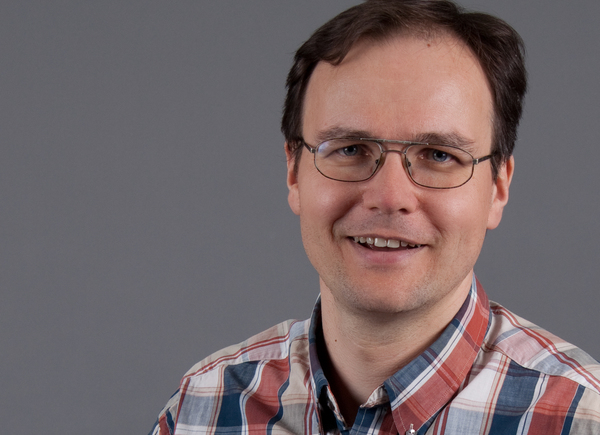
\includegraphics[width=0.9\linewidth]{assets/Stefan.jpeg}

\fontsize{6}{6}\selectfont
Prof. Dr. Stefan Naumann

\href{mailto:s.naumann@umwelt-campus.de}{s.naumann@umwelt-campus.de}

\vspace{0.5cm}

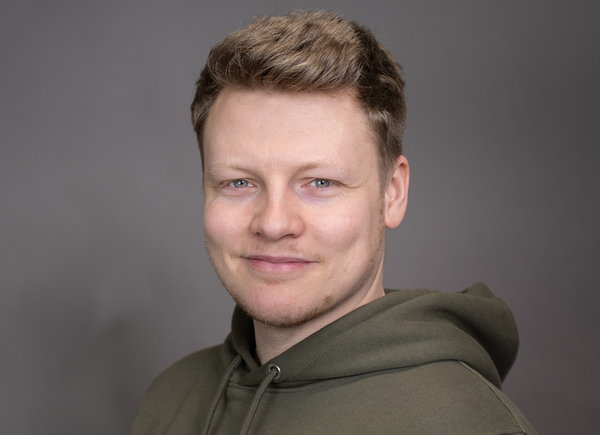
\includegraphics[width=0.9\linewidth]{assets/Sebastian.jpeg}

Sebastian Weber, M.C.Sc.

\href{mailto:seb.weber@umwelt-campus.de}{seb.weber@umwelt-campus.de}

\end{minipage}
\begin{minipage}{0.248\linewidth}

\vspace{0.2cm}

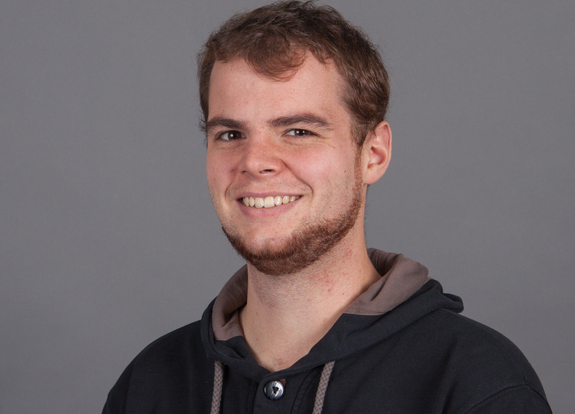
\includegraphics[width=0.9\linewidth]{assets/Achim.jpeg}

\fontsize{6}{6}\selectfont
Achim Guldner, M. Sc.

\href{mailto:a.guldner@umwelt-campus.de}{a.guldner@umwelt-campus.de}

\vspace{0.5cm}


\includegraphics[width=0.9\linewidth]{assets/max.jpeg}

Max Westing, B.A.

\href{mailto:m.westing@umwelt-campus.de}{m.westing@umwelt-campus.de}

\end{minipage}
\end{frame}



\end{document}